% !TeX root = ../main.tex
% Add the above to each chapter to make compiling the PDF easier in some editors.

\chapter{Method}\label{chapter:method}

%Previous skeletonization methods \cite{Shen2016}, \cite{Shen2017}, \cite{Ke2017}, \cite{Wang2019}, \cite{Xu2019} do not separate skeletons of multiple objects. Their prediction is a binary mask indiscriminately identifying skeleton points of all salient objects but its pertinent to separate skeletons of one object from another.
We propose a novel method for instance skeletonization in 3D biomedical images called Flux-and-Track. The method is partly motivated by DeepFlux~\cite{Wang2019} but differs in following ways: 
\begin{itemize}
	\item It separates skeletons for each individual segment - called as instance skeletonization.
	\item It is applied on 3D biomedical images instead of 2D images.
	\item After initial prediction, a splitting and matching step based on skeleton topology is devised to remove false merges and false splits.
\end{itemize}

Our Flux-and-Track method consists of three stages: 3D flux prediction using a
flux network, instance extraction and over-split skeleton generation, and finally
skeleton agglomeration by merging split skeletons. \autoref{fig:method_overview} depicts the overall pipeline and following sections explains the steps in details.

\begin{figure}[htpb]
	\centering
	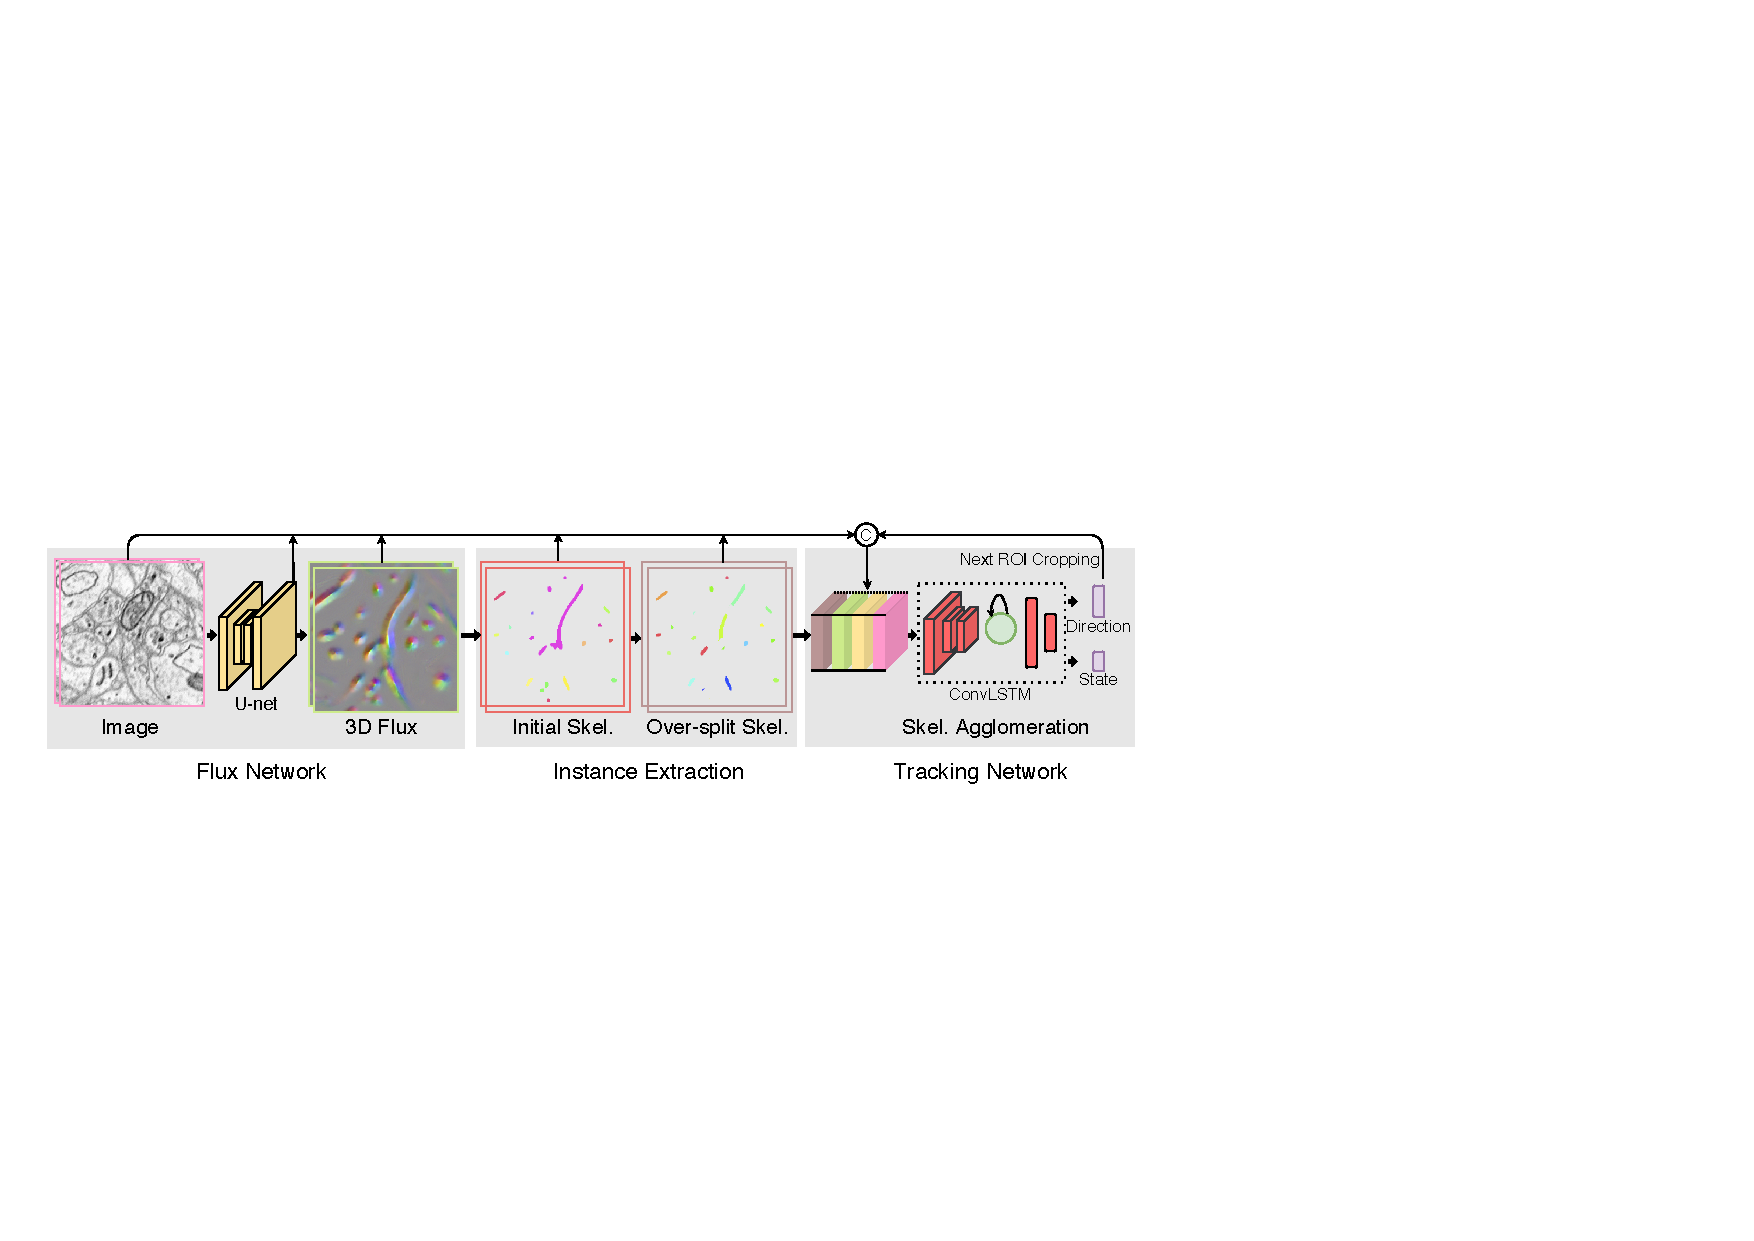
\includegraphics[width=\textwidth]{figures/model/architecture_0313.pdf}
	\caption{Overview of our Flux-and-Track method. The flux network takes raw image as input and outputs flux predictions. Next, the predicted flux goes through the instance extraction step to generate over-splitted instance proposals. Finally, we agglomerate the proposals based on predictions from the tracking network, namely the growing direction and \textit{continue}-\textit{stop} state. 
	}
	
	%  \yx{Make the caption more informative such that readers can fully understand the proposed method from this figure?
	%Weak skeleton regions often lead to false merge and false split errors for instance skeleton prediction.
	%Previously, (a) deep tracking methods are good at weak skeletons but computationally costly and (b) deep flux methods are efficient but not good at weak skeletons. (c) Our proposed method combines the strength of them.
	\label{fig:method_overview}
\end{figure}

%To achieve this, our proposed method encodes skeletons in a $\mathbb{R}^3$ vector field, similar to 'Deep Flux' \cite{Wang2019}, which encodes skeletons of objects in 2D images using a $\mathbb{R}^2$ vector field called \it{'flux'}. It also defines a 2D \it{context region} around skeleton, and all $\mathbb{R}^2$ flux vectors in that context region point to the nearest skeleton pixel, all remaining locations have zero 'flux'. The proposed method also utilizes the context region albeit in 3D, shown in \autoref{fig:context_field_directions}. Skeletons can be decoded from flux by finding 'sinks' of field, as all vectors of the field near a skeleton voxel will point towards it. While, \cite{Wang2019} uses a heuristic based algorithm for decoding, proposed method employs established methods - divergence and connected components - to extract skeletons.
%
%A second step of splitting skeletons is also proposed to rectify false merges and create an over split skele. This step of error detection and correction is similar in vein to \cite{Brain2019} and \cite{Seung2017}.
%For skeletons, merge and split locations can be identified with junction-points and end-points respectively. All branches are split at junction-points resulting in an over split version, which further can be agglomerated by matching nearby skeletons using their end-points and a learned binary classifier.

\section{Flux Network for 3D Flux Prediction}

\begin{figure}[t]
	\centering
	\captionsetup[subfigure]{justification=centering}
	\null\hfill
	\begin{subfigure}[c]{0.40\textwidth}
		\frame{\includegraphics[width=\textwidth]{figures/contextField/flux_vis_2.png}}
		\caption{\label{fig::context_field_directions_a}}
	\end{subfigure}
	\begin{subfigure}[c]{0.265\textwidth}
		\frame{\includegraphics[width=\textwidth]{figures/contextField/context.png}}
		\caption{\label{fig::context_field_directions_b}}
	\end{subfigure}
	\begin{subfigure}[c]{0.15\textwidth}
		\frame{\includegraphics[width=\textwidth]{figures/interpolation/field_ni.png}}
		\caption{\label{fig::context_field_directions_c}}
	\end{subfigure}
	\begin{subfigure}[c]{0.15\textwidth}
		\frame{\includegraphics[width=\textwidth]{figures/interpolation/field_i.png}}
		\caption{\label{fig::context_field_directions_d}}
	\end{subfigure}
	\hfill\null
	\caption{{\bf 3D skeleton context flux.} (a) Blue: a synthetic object segment, Purple: the skeleton; Green: context region of the skeleton; Red: flux vectors pointing away from the skeleton, (b) Neural skeletons and their context regions, (c) Color-coded flux field. Roughness due to discrete skeleton points (d) Smooth flux field after interpolating skeletons using splines. (Best viewed in electronic version).}
	\label{fig:context_field_directions}
\end{figure}

\subsection{Flux Definition}
We formulate skeleton prediction as a regression problem and define a 3D flux field from ground truth skeleton points $\Omega_s$ following the 2D flux representation in \cite{Wang2019}. Centered at each skeleton point, the {\it context region} $\Omega_c$ is defined as the set of points inside 3D balls of radius r centered at the skeleton points:

\DeclarePairedDelimiter\norm\lVert\rVert

\begin{equation}
\Omega_c= \{ \mathbf{x} : \min_{\mathbf{y} \in \Omega_s} \|\mathbf{x} - \mathbf{y}\|_2 < r \}
\end{equation}

Further a scalar distance function $D$ is defined from the skeleton points inside the domain $\Omega$ as follows:

\begin{equation}
\mathbf{D}(\mathbf{x}) := \begin{cases}
		\min_{\mathbf{y} \in \Omega_s} \norm{\mathbf{x}-\mathbf{y}}_2 & \text{if } \mathbf{x} \in \Omega_c \\
		0  & \text{otherwise}
		\end{cases} 
\end{equation}

Finally, flux $\overline{D}$, which is a $\mathbb{R}^3$ vector field is obtained by taking discrete gradient of $D$:

\begin{equation}
 \overline{\mathbf{D}}(\mathbf{x}) := \begin{cases}
 \nabla \mathbf{D} & \text{if } \mathbf{x} \in \text{int } \Omega_c \\
 0  & \text{otherwise}
 \end{cases} 
\end{equation}
 
In essence $\overline{\mathbf{D}}$ is a field with non-zero direction vectors defined in the {\it context region} of skeletons, such that the vectors are pointing away from the skeletons, as shown in~\autoref{fig:context_field_directions} (a).
	
But such flux is non-smooth if the skeletons are defined on a discrete grid, shown in \autoref{fig:context_field_directions} (c). Learning such a non-smooth field is not encouraged as deep convolutional networks usually fail to generate such sharp fields. Hence, to create smoother field ( \autoref{fig:context_field_directions} (d)), skeleton points are interpolated using splines and distance transform is computed using the interpolated points.

%\begin{figure}[htpb]
%	\newcommand{\mywidth}{0.22\textwidth}
%	\centering
%	\hspace{3mm}
%	\begin{subfigure}[b]{\mywidth}
%		\centering
%		\includegraphics[width=\textwidth]{data/images/interpolation/slice_edited.png}
%		\caption{\label{fig:3dseg_slice}}
%	\end{subfigure}
%	\hspace{3mm}
%	\begin{subfigure}[b]{\mywidth}
%		\centering
%		\includegraphics[width=\textwidth]{data/images/interpolation/linear_skel.png}
%		\caption{\label{fig:skel_linear}}
%	\end{subfigure}
%	\hspace{3mm}
%	\begin{subfigure}[b]{\mywidth}
%		\centering
%		\includegraphics[width=\textwidth]{data/images/interpolation/spline_skel.png}
%		\caption{\label{fig:skel_spline}}
%	\end{subfigure}\\
%	\hspace{3mm}
%	\begin{subfigure}[b]{\mywidth}
%		\centering
%		\includegraphics[width=\textwidth]{data/images/interpolation/seg_slice.png}
%		\caption{\label{fig:im_seg}}
%	\end{subfigure}
%	\hspace{3mm}
%	\begin{subfigure}[b]{\mywidth}
%		\centering
%		\includegraphics[width=\textwidth]{data/images/interpolation/dtx_linear.png}
%		\caption{\label{fig:dtx_linear}}
%	\end{subfigure}
%	\hspace{3mm}
%	\begin{subfigure}[b]{\mywidth}
%		\centering
%		\includegraphics[width=\textwidth]{data/images/interpolation/dtx_spline.png}
%		\caption{\label{fig:dtx_spline}}
%	\end{subfigure}\\
%	\hspace{\mywidth}
%	\hspace{3mm}
%	\begin{subfigure}[b]{\mywidth}
%		\centering
%		\includegraphics[width=\textwidth]{data/images/interpolation/gradz_linear.png}
%		\caption{\label{fig:grad_linear}}
%	\end{subfigure}
%	\hspace{3mm}
%	\begin{subfigure}[b]{\mywidth}
%		\centering
%		\includegraphics[width=\textwidth]{data/images/interpolation/gradz_spline.png}
%		\caption{\label{fig:grad_spline}}
%	\end{subfigure}
%	\caption{ \subref{fig:skel_linear} and \subref{fig:skel_spline} are resulting skeletons for linearly and spline interpolation methods respectively. \subref{fig:im_seg} is a segment slice in $X-Y$ plane sliced as shown in \subref{fig:3dseg_slice}. \subref{fig:dtx_linear} and \subref{fig:dtx_spline} are the normalized isotropic 3D distance transform from the skeleton for linearly and spline interpolated versions respectively. \subref{fig:grad_linear} and \subref{fig:grad_spline} shows the $z$ component of the gradient of \subref{fig:dtx_linear} and \subref{fig:dtx_spline} respectively. Sharp fields exist in \subref{fig:grad_linear} due to artifacts in the distance transform in \subref{fig:dtx_linear}.}
%	\label{fig:splineInterpolation}
%\end{figure}


The advantages for encoding skeletons in such a field are:
\begin{itemize}
	\item Flux Network has to learn to look for both global and local properties while predicting the field. This helps to avoid local false merges
	\item Voxel wise loss function for the deep net can be easily constructed and the training objective can be agnostic of the number of skeleton instances.
	\item Predicted field can be useful to solve false merges and splits in later post processing steps.
\end{itemize}


\subsection{Network Design}
Since flux field representation is non-local and highly dependent on underlying 3D shapes we use a fully convolutional 3D U-net to predict the 3D flux field from 3D images to enable versatile representations from the training objects. Details about the network architecture are shown in the appendix (\autoref{fig:flux_net}).

\subsection{Training Objective}

\begin{equation}\label{eqn:cosineLoss}
\mathcal{L}_{cos}(\mathbf{P}, \mathbf{T}) := \sum_{\mathbf{x} \in \Omega} \mathbf{W}(\mathbf{x})\left( 1 - \frac{\mathbf{P}(\mathbf{x}).\mathbf{T}(\mathbf{x})}{\max(\norm{\mathbf{P}(\mathbf{x})}_2.\norm{\mathbf{T}(\mathbf{x})}_2,\,\epsilon)} \right)
\end{equation}

\begin{equation} \label{eqn:mse}
\mathcal{L}_{mse}(\mathbf{P}, \mathbf{T}) := \sum_{\mathbf{x} \in \Omega} \mathbf{W}(\mathbf{x}) \norm{ \norm{\mathbf{P}(\mathbf{x})}_{2} - \norm{\mathbf{T}(\mathbf{x})}_{2}}_2^2
\end{equation}

\begin{equation} \label{eqn:fluxLoss}
\mathcal{L}_{flux} := \alpha\mathcal{L}_{cos} + (1-\alpha)\mathcal{L}_{mse}
\end{equation}

Though a L2 or L1 loss between target field $\mathbf{T}$ and predicted field $\mathbf{P}$ can be used, but a more stringent loss would be to enforce correct prediction of the directions of the vectors, hence weighted cosine similarity is used to calculate the loss (\autoref{eqn:cosineLoss}). This forces a sharper prediction and ensures that the network directly learns directions and hence the shape of the neurons. Weight $\mathbf{W}$ balances the loss contribution from context and non-context regions, defined as $|\overline{\Omega_{c}}|/|\Omega_{c}|$ for context region and 1 otherwise. Since, outside skeleton context region the vector field has zero magnitude and therefore cosine loss is meaningless, a weighted combination (\autoref{eqn:fluxLoss}) of mean square error (\autoref{eqn:mse}) and cosine loss (\autoref{eqn:cosineLoss}) is used. \autoref{fig:learnedField} shows the learned flux prediction.

\begin{figure}[t]
	\newcommand{\mywidth}{0.24\textwidth}
	\centering
	\begin{subfigure}[b]{\mywidth}
		\centering
		\includegraphics[width=\textwidth]{data/images/fieldLearning/fi_image.png}
		\caption{\label{fig:fi_im}}
	\end{subfigure}
	\begin{subfigure}[b]{\mywidth}
		\centering
		\includegraphics[width=\textwidth]{data/images/fieldLearning/fi_im_field.png}
		\caption{\label{fig:fi_im_f}}
	\end{subfigure}
	\begin{subfigure}[b]{\mywidth}
		\centering
		\includegraphics[width=\textwidth]{data/images/fieldLearning/fi_field.png}
		\caption{\label{fig:fi_f}}
	\end{subfigure}
	\begin{subfigure}[b]{\mywidth}
		\centering
		\includegraphics[width=\textwidth]{data/images/fieldLearning/fi_result.png}
		\caption{\label{fig:fi_r}}
	\end{subfigure}
	
	\caption{\subref{fig:fi_im} and \subref{fig:fi_f} shows an 2D slice of input data and the ground truth field. They are overlayed in \subref{fig:fi_im_f}. \subref{fig:fi_r} shows the predicted field.}
	\label{fig:learnedField}
\end{figure}

\section{Instance Extraction for Over-split Skeletons}
To obtain the instance skeletons back from such an encoding, a simple postprocessing step is devised. First observation about the predicted field is: in the vicinity of skeleton voxels they point away from each other, while at non skeleton voxels they point almost in the same direction. This property can be used to identify skeleton voxels, {\it divergence} at skeleton points would be high, where as for all other locations it would be low. Thus, thresholding the {\it divergence} would allow to create a skeleton mask. For separating skeletons of different instances connected components analysis can be performed.

\subsection{Topological Skeleton Graph}
We thin the predicted skeletons to a single voxel width and create an undirected graph, shown in~\autoref{fig:method_proposal}~(b). Based on the degree of incident edges, we can identify the vertices $V$ into junctions ${J := \{n \in V : \text{degree}(n) > 2\}}$ and endpoints ${E := \{n \in V : \text{degree}(n) = 1\}}$.

\subsection{Generating Over-split Skeletons}
While connected component analysis separates skeleton instances of most segments, but closely located skeletons crossing each other could be falsely merged. This would create junctions unless skeletons of two parallel segments are merged throughout which is unlikely. So we utilize the topological skeleton graph to split skeletons at junctions $J$ (\autoref{fig:method_proposal}). Predicted skeletons are split by partitioning with a plane as orthogonal as possible to the merged skeletons. Such a plane can be defined using Singular Value Decomposition of all skeletons points near the junction. 

This process creates over-split skeletons (\autoref{fig:method_proposal} (c)) which can be agglomerated using another post-processing step.

\begin{figure}[t]
	\newcommand{\hwidth}{0.32\textwidth}
	\captionsetup[subfigure]{aboveskip=1pt,belowskip=1pt}
	\centering
	\begin{subfigure}[b]{\hwidth}
		\frame{\includegraphics[width=\textwidth]{figures/splitNMerge2/sm_initial.png}}
		\caption{\label{fig:method_proposal_a}}
	\end{subfigure}
	\begin{subfigure}[b]{\hwidth}
		\frame{\includegraphics[width=\textwidth]{figures/splitNMerge2/sm_initial_topology.png}}
		\caption{\label{fig:method_proposal_b}}
	\end{subfigure}
	\begin{subfigure}[b]{\hwidth}
		\frame{\includegraphics[width=\textwidth]{figures/splitNMerge2/sm_split_topo_ends.png}}
		\caption{\label{fig:method_proposal_c}}
	\end{subfigure}
	\caption{{\bf Over-split skeletons.} (a) Thick and falsely merged predicted skeletons (b) Topological graph constructed by thinning and identified junction point (c) Result of splitting skeletons at junction point}
	\label{fig:method_proposal}
	\vspace{-0.1in}
\end{figure}

%\begin{figure}[htpb]
%	\newcommand{\mywidth}{0.3\textwidth}
%	\centering
%	\begin{subfigure}[b]{\mywidth}
%		\centering
%		\includegraphics[width=\textwidth]{data/images/splitting/junction.png}
%		\caption{\label{fig:skelSplitA}}
%	\end{subfigure}
%	\hspace{3mm}
%	\begin{subfigure}[b]{\mywidth}
%		\centering
%		\includegraphics[width=\textwidth]{data/images/splitting/plane.png}
%		\caption{\label{fig:skelSplitB}}
%	\end{subfigure}
%	\hspace{3mm}
%	\begin{subfigure}[b]{\mywidth}
%		\centering
%		\includegraphics[width=\textwidth]{data/images/splitting/split.png}
%		\caption{\label{fig:skelSplitC}}
%	\end{subfigure}
%	\caption{Splitting of skeletons. \subref{fig:skelSplitA} shows two crossing skeletons which are falsely merged at the yellow junction point. \subref{fig:skelSplitB} shows the cutting plane which is thickened and skeletons voxels inside it deleted. \subref{fig:skelSplitC} shows the resulting over-split skeletons.}
%	\label{fig:skelSplit}
%\end{figure}

%Splitting would create an over-split skeletons with almost no false merges, hence to improve upon such, a merging step is devised. A classifier is trained to predict if a pair of skeletons can be merged. To find such pairs, all possible permutations of end point pairs, which are within a threshold distance are found. \cite{Brain2019} proposes a similar idea where skeleton directions at end point are also used to decide if segmentations can be merged. End point directions are not used here because pruning possible matches based on directions can also remove correct combinations. Instead, directly delegating the task to a learned classifier is more straightforward and error free, hoping that it should learn direction consistency and other cues using the training examples as shown in \autoref{fig:skelMatchTrainData}. The classifier would have to learn if based on the vector field, EM image and the existing two skeleton masks should they be merged. 
%
%The input to the classifier are: 1) A cropped 3D volume of EM image around the center of the two end points of the skeleons. 2) A cropped mask of skeletons in two separate channels. 3) And the cropped predicted vector field. The output of the classifier is a scalar probability score which is thresholded to get a binary output. \autoref{fig:skelSplitNMatch} shows the workflow of split and merge method discussed above.
%
%\begin{figure}[htpb]
%	\centering
%	\begin{subfigure}[b]{0.3\textwidth}
%		\centering
%		\includegraphics[width=\textwidth]{data/images/matchingData/positive_2.png}
%		\caption{\label{fig:positiveMatch}}
%	\end{subfigure}
%	\hspace{3mm}
%	\begin{subfigure}[b]{0.3\textwidth}
%		\centering
%		\includegraphics[width=\textwidth]{data/images/matchingData/negative_2.png}
%		\caption{\label{fig:negativeMatch}}
%	\end{subfigure}
%	\caption{Positive \subref{fig:positiveMatch} and negative \subref{fig:negativeMatch} training samples for training a classifier to merge skeletons. Each red line in \subref{fig:negativeMatch} pairs two skeletons which are not part of the same segment. Green line in \subref{fig:positiveMatch} represent the skeleton parts from same segment which needs to be matched. The dark green region is the context region of the skeleton.}
%	\label{fig:skelMatchTrainData}
%\end{figure}
%
%\begin{figure}[htpb]
%	\centering
%	\begin{subfigure}[b]{0.24\textwidth}
%		\centering
%		\includegraphics[width=\textwidth]{data/images/splitNMatch/skel.png}
%		\caption{\label{fig:splitNMatchA}}
%	\end{subfigure}
%	\hfill
%	\begin{subfigure}[b]{0.24\textwidth}
%		\centering
%		\includegraphics[width=\textwidth]{data/images/splitNMatch/skelNSeg.png}
%		\caption{\label{fig:splitNMatchB}}
%	\end{subfigure}
%	\hfill
%	\begin{subfigure}[b]{0.24\textwidth}
%		\centering
%		\includegraphics[width=\textwidth]{data/images/splitNMatch/split.png}
%		\caption{\label{fig:splitNMatchC}}
%	\end{subfigure}
%	\hfill
%	\begin{subfigure}[b]{0.24\textwidth}
%		\centering
%		\includegraphics[width=\textwidth]{data/images/splitNMatch/matched.png}
%		\caption{\label{fig:splitNMatchD}}
%	\end{subfigure}
%	\caption{Splitting and matching of skeletons. \subref{fig:splitNMatchA} and \subref{fig:splitNMatchB} shows the falsely merged skeletons. \subref{fig:splitNMatchC} shows skeletons after splitting. Notice that the colors of the skeletons have changed. \subref{fig:splitNMatchD} shows the classifier linking the correct skeletons parts together with yellow lines.}
%	\label{fig:skelSplitNMatch}
%\end{figure}

\section{Tracking Network for Skeleton Agglomeration}

\subsection{Network Design}
To iteratively grow and merge skeletons from endpoints, we train a 3D Conv-LSTM-FC based recurrent tracking network (\autoref{fig:method_overview}). While growing, if the predicted trajectory hits another skeleton, both skeletons are merged together. Every growing step produces two outputs: first, the direction along which the skeleton is to be grown, which is scaled by a constant $\lambda$ to jump to the next position; second, a binary state variable ${\textit{\{continue-stop\}}}$ controlling if the growing should be terminated at current position.  
The input to the network is a small ROI from previous layers, initially centered at a skeleton end and moved as the tracking proceeds. The layers consist of the image, skeleton mask and Flux Net features which provides a larger spatial context to the Tracking Network. Details about the network architecture is shown in the appendix (\autoref{fig:direction_net}).


\subsection{Loss Functions}
We use the predicted over-split skeletons from the Flux Network as seeds and ground truth skeleton graph $G_{gt}$ to find a path between pairs of over-split skeleton segments. 
To minimize the influence from artifacts stemming from all the stages, including annotation, thinning and smoothing (\autoref{fig:method_skel_agg} (a)), ground truth skeletons only provides guidance for tracking. Starting from an end point, an oracle can track by only utilizing directions from nearest nodes in the ground truth skeleton graph, shown in \autoref{fig:method_skel_agg} (b). These on-the-fly directions supervise the learning of our Tracking Network.

We want our predictions to follow the ground truth (GT) path smoothly and loosely without running astray. Therefore, at every step, we dynamically calculate the target direction $\mathbf{u_t}$ using the tangential direction from multiple closest GT nodes and also the normal direction to the GT path.
The target state $s_t$ is \textit{continue} until the model tracks till the corresponding split skeleton pair or reaches the GT graph end. We define loss functions for directions and path states as follows: 
\begin{align}
\mathcal{L}_{\text{dir}, \Tilde{t}}&= \sum_{t=\Tilde{t}}^{\Tilde{t} + \frac{N}{2}} \left( 1 - \frac{\mathbf{u_t}.\mathbf{v_t}}{\max(\|\mathbf{u_t}\|_2.\|\mathbf{v_t}\|_2,\,\epsilon)} \right), \label{eqn:dirLoss}\\
\mathcal{L}_{\text{state}, \Tilde{t}}&= \sum_{t=\Tilde{t}}^{\Tilde{t} + \frac{N}{2}} w_t \left( -s_t\log(r_t) - (1-s_t)\log(1-r_t) \right). \label{eqn:stateLoss}\\
\mathcal{L}_{\text{track}, \Tilde{t}} &= \mathcal{L}_{dir, \Tilde{t}} + \beta\mathcal{L}_{state, \Tilde{t}}\label{eqn:trackingLoss}\\
w_t&= \begin{cases}
1  & \text{if } s_t = \text{\textit{continue}} \\
t & \text{if } s_t = \text{\textit{stop}}
\end{cases}\label{eqn:trackingWeight}
\end{align}
We use cosine similarity (~\autoref{eqn:dirLoss}) as a training loss for directions and weighted binary cross entropy (\autoref{eqn:stateLoss}) for path states. To avoid the tracking going astray during initial epochs, we perform multiple-phase training with increasing max steps of $N=\{4, 8, 16, 32\}$ and optimize the tracking loss every $\frac{N}{2}$ steps.

\begin{figure}[t]
	\newcommand{\hwidth}{0.32\textwidth}
	\captionsetup[subfigure]{aboveskip=1pt,belowskip=1pt}
	\centering
	\begin{subfigure}[b]{\hwidth}
		\frame{\includegraphics[width=\textwidth]{figures/splitNMerge2/sm_split_gt_topo.png}}
		\caption{\label{fig:method_skel_agg_a}}
	\end{subfigure}
	\begin{subfigure}[b]{\hwidth}
		\frame{\includegraphics[width=\textwidth]{figures/splitNMerge2/sm_seg_gt_oracle_paths_arrow_1.png}}
		\caption{\label{fig:method_skel_agg_b}}
	\end{subfigure}
	\begin{subfigure}[b]{\hwidth}
		\frame{\includegraphics[width=\textwidth]{figures/splitNMerge2/sm_merged_e.png}}
		\caption{}
		\label{fig:method_skel_agg_c}
	\end{subfigure}
	%\caption{Skeleton agglomeration. (a) shows ground truth skeletons which do not align perfectly with the predicted skeletons (b) shows oracle generated tracking paths obtained by using ground truth skeleton directions as guidance (c) shows predicted paths from Deep Tracking Net connecting correct skeleton pairs.}
	\caption{Skeleton agglomeration. (a) Misaligned predicted and ground truth skeletons. (b) Oracle generated tracking paths using ground truth skeleton directions as guidance (c) Over-split skeleton pairs correctly agglomerated by Tracking Network.}
	\label{fig:method_skel_agg}
	\vspace{-0.1in}
\end{figure}

\section{End-to-End Fine Tuning}
Initially, we train the flux network and the tracking network separately for the dependency relationship between two networks. We perform final fine-tuning end-to-end by jointly optimizing linear combination of all losses as shown in \autoref{eqn:totalLoss}.
\begin{align}
     \mathcal{L}= \alpha\mathcal{L}_{cos} + \beta\mathcal{L}_{scale} + \gamma\mathcal{L}_{dir, \Tilde{t}} + \phi\mathcal{L}_{state, \Tilde{t}}.\label{eqn:totalLoss}
     %\mathcal{L}= \mathcal{L}_{\text{flux}} + \gamma\mathcal{L}_{\text{track}, \Tilde{t}}\label{eqn:totalLoss}
\end{align}

The scaling constants $\alpha, \beta, \gamma, \phi$ are determined empirically and satisfy the constraint: $\alpha+\beta+\gamma+\phi = 1$. 

\section{Data Augmentation}
Augmenting 3D data while training has been very effective in improving affinity prediction for EM segmentation \cite{Zeng2017, Kisuk2017}. Borrowing the training set augmentations from previous methods \cite{Kisuk2017, ELEKTRONN}, the following augmentations were applied for Flux Network.
\begin{itemize}
	\item \textbf{Rotations} of $90^{\circ}$ degree and also incremental along Z axis.
	\item \textbf{Flips} in $x$, $y$ and $z$ dimensions.
	\item \textbf{Rescaling} images, skeleton and subsequently the field which was done prior to training.
	\item \textbf{Gaussian blur} of a random set of $2D$ slices in input volume. This mimics the actual scenario when only a few slices are out-of-focus and intermittently spread in $3D$.
	\item \textbf{Elastic deformation} of images. A random perturbing field is defined in such a way that the images are only slightly deformed with a max of 6 pixels, which would not significantly move skeletons. Hence, this can be done on-the-fly during training. This augmentation can force the network to look for 3D shape features rather than focusing entirely on boundaries.
	\item Random \textbf{brightness}, \textbf{contrast} adjustments and \textbf{gamma-correction}.
	\item \textbf{Missing parts}, where a random part of the $2D$ slice is replaced with a flat grayscale value. This mimics artifacts in $2D$ slices due to physical folding, knife marks etc.
	\item \textbf{Missing section}, where few $2D$ slices are removed from the input stack. This mimics the case when few slices are lost and not imaged due to other issues. This causes a discernible discontinuity along $Z$ axis.
	\item \textbf{Misalignment}, where a few randomly chosen slices are displaced laterally by few pixels. Which can occur in a real scenario when alignment is not perfect due to image artifacts. 
\end{itemize}

For Tracking Network only $90^{\circ}$ Rotations, Flip and Transpose augmentation operations were used.